
\begin{comment}
\begin{titlepage}
\maketitle
\end{titlepage} 
\end{comment}

%% \begin{comment}
\begin{titlepage}
\begin{center}
%% Upper part of the page
%\includegraphics[width=1\textwidth]{./up-logo.jpg}\\[0.4cm]    
\textsc{\LARGE Primeira Edição}\\[1.0cm]
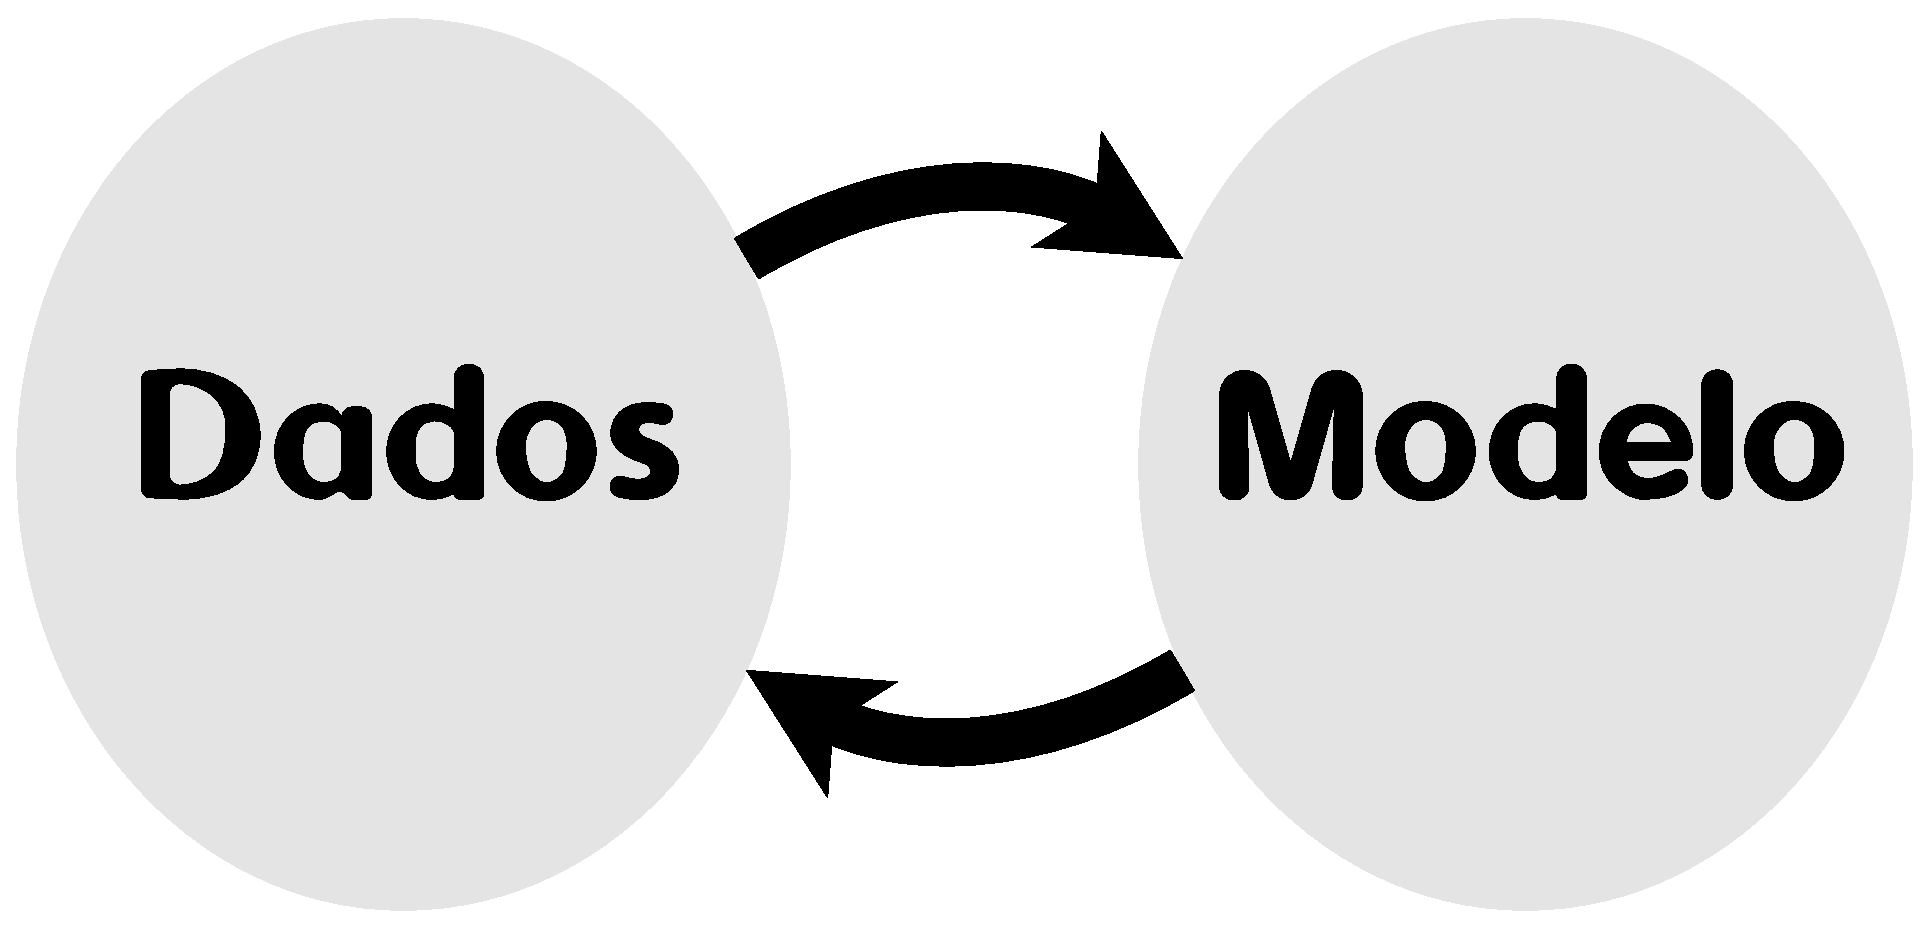
\includegraphics[width=0.6\textwidth]{principal}\\[1.0cm]
%% pretitle
%{\fontsize{25}{30} \textsc{Algum pretitulo}}
%% Title
\HRule{0.4cm} \\[0.4cm]
{ \fontsize{50}{60}   \bfseries \mytitle}\\[0.4cm]
\HRule{0.4cm} \\[0.7cm]
%% SubTitle
{\fontsize{25}{30} \textsc{\mysubtitle}}\\[0.5cm]
\vfill
%% Author 
\textsc{\LARGE  \myauthor }
\begin{comment}
\begin{minipage}{0.4\textwidth}
\begin{flushleft} \large
%\emph{Author:}\\
\myauthor %\textsc{Coppejans}
\end{flushleft}
\end{minipage}
% ID
\begin{minipage}{0.4\textwidth}
\begin{flushright} \large
\emph{email:} \\
\ImprimirEmail
\end{flushright}
\end{minipage}
\end{comment}
% Bottom of the page
\vfill
\textsc{\LARGE Lavras/MG}\\[0.4cm]
\textsc{\LARGE \imprimiryear}
\end{center}
\end{titlepage}
%% \end{comment}
